
\section{Q5 - Resultados Globais}

Após o scan feito pelo OpenVass obtivemos os seguintes dados.

\begin{figure}[H]

  \centering

  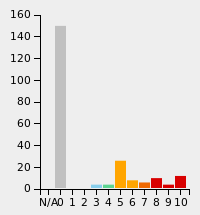
\includegraphics[scale = 0.45]{graphChart.png}

  \caption {Gravidade das vulnerabilidades encontradas}

  \label {fig1}

\end{figure}

Nesta figura podemos observar o número de vulnerabilidades conhecidas e atualmente na base de dados do OpenVass encontradas no Metasploite2.
Em seguida apresentam-se as vulnerabilidades encontradas no Sistema visado.

\subsection{Apache HTTP Server}

\par O servidor avaliado corre com um servidor Apache HTTP e está vulnerável a permitir acesso a informação sensivel através das cookies. O error ocorre devido á resposta de erro por defeito com código de estado 400, quando não é configurado um documento personalizado de erro.
\par Isto pode levar a que um atacante consiga obter informação sensivel que possa auxiliar num ataque futuro.
\par Pode ser facilmente corrigido atualizando para uma versão 2.2.22 ou posterior.

\subsection{phpMyAdmin}

O servidor está a correr phpMyAdmin e é vulnerável a cross-site scripting. Isto permite que atacantes conduzam ataques com injeção de código HTML arbitrário para gerar ataques de phishing.
\par Ainda não foi criada uma solução e provavelmente nenhuma será criada. Deve-se mudar o serviço ou desabilitar a resposta.


\subsection{Samba MS-RPC}

\par Esta vulnerabilidade permite que atacantes executem comandos arbitrários na shell. Com isto o atacante pode correr comandos na shell com as permissões da aplicação.
\par Para corrigir isto basta fazer uma atualização do software usado.

\subsection{PostGreSQL}

Podia-se aceder a uma base de dados PostgreSQL ao usar credenciais fracas, nomeadamente com a password "postgres".
\par Para evitar acessos indevidos deve-se redifinir a palavra pass o mais cedo possível. 


\subsection{VNC Brute Force Login}

\par Este método passa por tentar aceder como uma password dada via protocolo VNC, a password usada é password.
\par Basta substituir a password por uma mais dificil.


\subsection{DistCC}

\par Esta vulnerabilidade passa por aproveitar a falta de resrições nos acessos ás portas do servidor, dado que o DistCC confia cegamente nos clientes. Um atacante pode simplesmente correr comandos arbitrários no servidor.
\par Este problema resolve-se fazendo uma atualização do software.


\subsection{Distributed Ruby}

\par Esta falha permite que sistemas não autorizados executem comandos distribuidos, isto pois o Distributed Ruby não previne atividades de acesso priviligiado, caso este corra com acesso priviligiado um atacante pode executar comandos ou scripts ruby.
\par Para colmatar a falha basta restringir as permissões do serviço caso se permita o acesso a utilizadores não confiaveis ou então definir ACLs apropriadas no sistema.


\subsection{Ingreslock}

\par Uma backdoor é instalado no sevidor remoto. O serviço responde a um id: uid=0, gid=0. Com isto um atacante pode executar código arbitrário com privilégios "root".
\par Não há correção disponivel para esta vulnerabilidade.




\section{Q6 - Tráfego Anómalo}

Nesta secção serão analisados dois exemplos de tráfego anómalo reportados pelo Snort.

\subsection{PROTOCOL - SNMP AgentX/tcp request}

\par O 5º pacote identificado pelo Snort corresponde ao pacote número 233 do WireShark.
\par Este pacote corre sobre TCP e tem origem no endereço: 172.16.1.128, porta: 46754 destinando-se ao endereço: 172.16.1.129, porta: 80.

\subsubsection{CVE-2002-0012}

\begin{figure}[H]

  \centering

  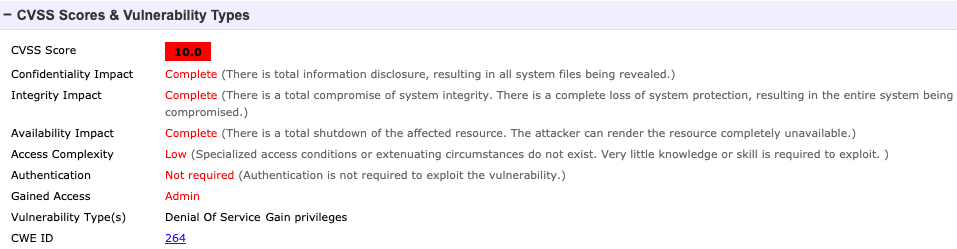
\includegraphics[scale = 0.45]{CVE-2002-0012.png}

  \caption {CVE-2002-0012}

  \label {fig2}

\end{figure}

\par Definição: Há vulnerabilidades num grande número de implementações do SNMP que permitem que atacantes possam efetuar ataques de denial of Service ou ganhar privilégios via uma armadilha SNMPv1.

\par Modo de proceder: O atacante provoca um erro cujo estado seja 400. Devido a um erro na criação de um documento personalizado este pode ser explorado para expor "httpOnly" cookies.

\subsection{FTP Command Overflow Attempt}

\par O 13º pacote identificado pelo Snort corresponde ao pacote número 9484 do WireShark.
\par Este pacote corre sobre TCP fazendo uso de FTP e tem origem no endereço: 172.16.1.128, porta: 56385 destinando-se ao endereço: 172.16.1.129, porta: 21.
\par De seguida apresenta-se o CVE mais recente relacionado com este problema.

\subsubsection{CVE-2007-0019}

\begin{figure}[H]

  \centering

  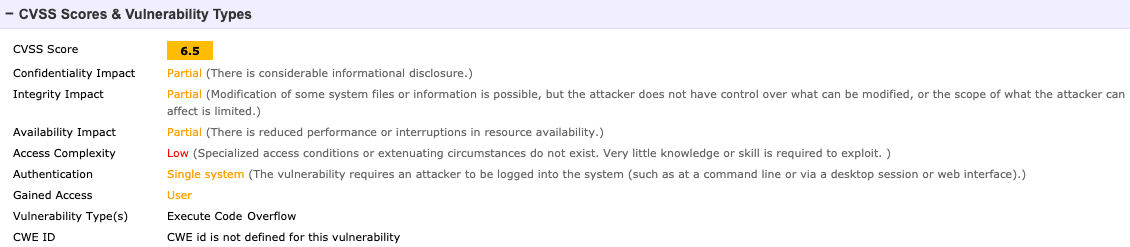
\includegraphics[scale = 0.45]{CVE-2007-0019.png}

  \caption {CVE-2002-0012}

  \label {fig2}

\end{figure}

\par Definição: O atacante executa código arbitrário fazendo uso de um comando LIST longo e outros pedidos ao serviço FTP permitindo que estes executem código arbitrário com pedidos não especificados ao serviço HTTP.



\section{Q7 - Vulnerabilidades Snort vs OpenVass}

\begin{itemize}
\item A principal razão para o Snort apresentar vulnerabilidades que o openVas não reporta deve-se aos falsos positivos.
\par Há comportamentos reconhecidos como tráfego anómalo, por exemplo um "port scan" feito por um administrador da rede. O Snort vai detetar este tráfego e sinaliza-lo como tal, no entanto não se trata de uma tentativa de intrusão. Já o OpenVass não reporta este scan visto que apenas reporta falhas anómalos como por exemplo a utilização do serviço regexd sem ser sobre ssh que permite o envio de passwords em texto limpo.   

\item Uma razão pela qual o Snort pode apresentar mais falhas do que o OpenVas trata-se de o OpenVas trabalhar sobre aplicações e o Snort sobre a camada de rede. Assim o Snort pode reportar vários pacotes com comportamento anómalo como um "port scan", no entanto estes pacotes não representam necessáriamente a tentativa de exploração de uma falha pois por exemplo este scan pode ter sido feito pelo administrador da rede. Já o OpenVass deteta e reporta uma falha numa aplicação ou serviço no qual este fornece de alguma forma manipulação ou obtenção de informação sensivel.

\end{itemize}
\section{Q8 - Correção de vulnerabilidades}

\par Para visualização da correção das falhas alvo, note-se que o OpenVass faz um scan seguindo sempre a mesma ordem de teste portanto após a indicação de como foi corrigida cada falha aparecerá uma imagem com o antes e o depois das correções e vendo a falha anterior á falha alvo e a posterior constatar-se-á que a falha a ser corrigida foi de facto colmatada.

\subsection{HTTP Debugging Methods (Trace/Track) Enabled}

\begin{itemize}
\item Descrição da Vulnerabilidade: O servidor Web permite metodos de rastreamento HTTP que são usados para corrigir conecções ao servidor web.
Neste caso o método ativo é o TRACE. Com esta vulnerabilidade o atacante pode enganar o sistema fazendo com que este lhe envie as suas credencias.

\item Método de resolução: Basta desabilitar o uso do Trace para corrigir esta vulnerabilidade.

\par Para proceder á correção do problema primeiro foi preciso encontrar o ficheiro do apache2 responsável por desabilitar o trace, este ficheiro chama-se \textit{httpd.conf} e está localizado em \textit{/etc/apache2/}.
\par Em seguida abriu-se este ficheiro recorrendo ao comando nano como superuser: \textit{sudo nano httpd.conf} e escreveu-se o seguinte no ficheiro: \textit{TraceEnable Off}.

\begin{figure}[H]

  \centering

  \hbox{\hspace{-6em} 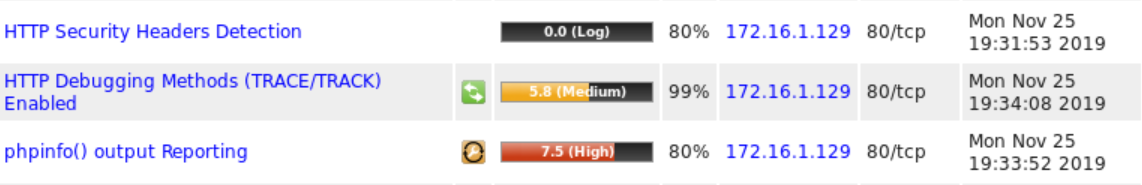
\includegraphics[scale = 0.4]{beforeHTTP.png}}

  \caption {HTTP Debugging Methods (Trace/Track) Enabled}

  \label {fig3}

\end{figure}
\begin{figure}[H]

  \centering

  \hbox{\hspace{-6em} 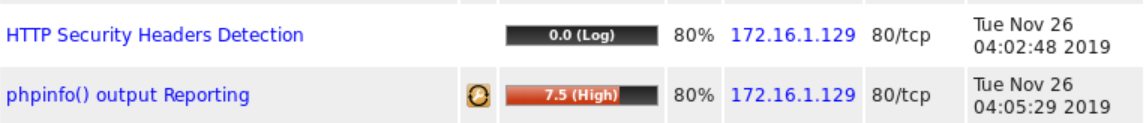
\includegraphics[scale = 0.4]{afterHTTP.png}}

  \caption {HTTP Debugging Methods (Trace/Track) Disabled}

  \label {fig3}

\end{figure}
\item Vulnerabilidades extra corrigidas:
\end{itemize}

\subsection{Rexecd Service Detection}

\begin{itemize}
\item Descrição da Vulnerabilidade: Este serviço permite a execução de comandos na shell de um computador remoto. N o entanto o rexec permite a autenticação lendo o username e password desencriptados da socket.

\item Método de resolução: Desabilitar o uso do serviço rexec e usar alternativas como o SSH.
\par Para realizar isto temos de ir até á pasta /etc, nesta abrimos com o comando \textit{sudo nano inetd.conf} o ficheiro inetd.conf e alteramos a linha: \textit{exec   stream    tcp  nowait  root /urs/sbin/tcpd  /usr/sbin/in.rexecd} para \textit{exec   stream    tcp  nowait  root /urs/sbin/sshd  /usr/sbin/in.rexecd}.
\par Isto fará com que este serviço inicie o servidor rexecd usando ssh. 
\begin{figure}[H]

  \centering

  \hbox{\hspace{-6em} 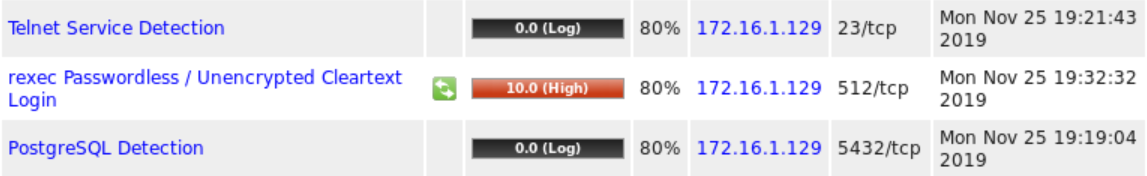
\includegraphics[scale = 0.4]{afterRexecd.png}}

  \caption {Rexecd Service over tcpd}

  \label {fig3}

\end{figure}
\begin{figure}[H]

  \centering

  \hbox{\hspace{-6em} 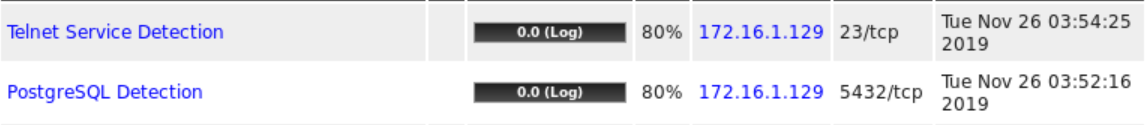
\includegraphics[scale = 0.4]{beforeRexecd.png}}

  \caption {Rexecd Service over sshd}

  \label {fig3}

\end{figure}
\item Vulnerabilidades extra corrigidas:
\end{itemize}

\subsection{Bind Shell Backdoor Detection}

\begin{itemize}
\item Descrição da Vulnerabilidade: Há uma possivel backdoor instalada no servidor remoto. Ocomando está a responder a um id=0(root) e gid=0(root). Um atacante pode executar um comando no contexto da aplicação e comprometer o sistema.

\item Método de resolução: Existem 3 métodos de corrigir esta vulnerabilidade.

\par\item Verificar se o servidor foi comprometido e reinstalar o sistema se necessário. 
\par\item Desativar o ingreslock.
\par O método aplicado é o bloqueio do inicio do serviço simplesmente comentando a linha \textit{ingreslock stream tcp nowait root /bin/bash bash -i}.
\begin{figure}[H]

  \centering

  \hbox{\hspace{-6em} 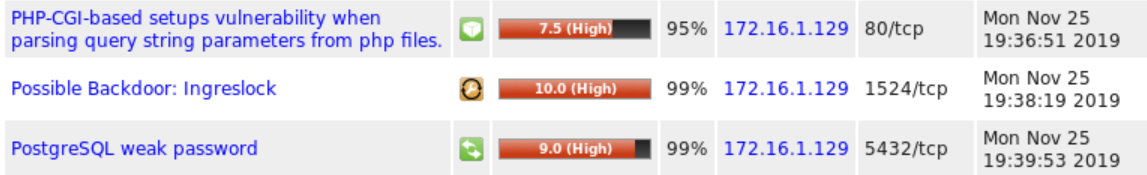
\includegraphics[scale = 0.4]{beforeBackdoor.png}}

  \caption {Ingreslock backdoor enabled}

  \label {fig3}

\end{figure}
\begin{figure}[H]

  \centering

  \hbox{\hspace{-6em} 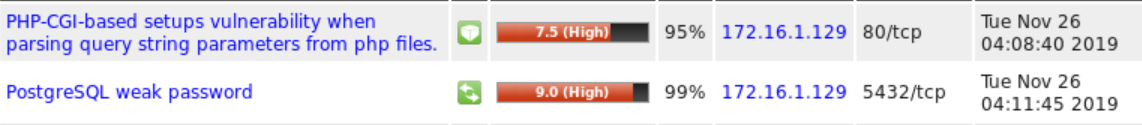
\includegraphics[scale = 0.4]{afterBackdoor.png}}

  \caption {Ingreslock Service not started}

  \label {fig3}

\end{figure}
\item Vulnerabilidades extra corrigidas:
\end{itemize}

\subsection{VNC Server ‘password’ Password}


\begin{itemize}
\item Descrição da Vulnerabilidade:O servidor VNC a correr no computador remoto utiliza uma password fraca, por defeito esta password é 'password'. Um atacante pode tirar partido disto para obter controlo sobre o sistema.
\par Note-se que antes de podermos corrigir o a falha do VNC tivemos de o inicializar com o comando: \textit{sudo vcnserver}. Isto pois o VCN estava mal inicializado, posteriormente foi criado um ficheiro \textit{passwd} em \textit{/home/msfadmin/.vnc/} onde foi colocada a nova password do vnc.

\item Método de resolução: Alterar a palavra pass para uma forte.
\par Para proceder á geração de uma password forte utilizamos um gerador online com 16 caracteres. A password obtida foi: \textit{5?V=X\#\&kAdB'H6+y}, infelizmente o vnc tem as password truncadas para 8 caracteres automáticamente, assim a password usada foi: \textit{5?V=X\#\&k}.\newline
\textit{Nota:} Como as passwords do VNC são truncadas para 8 caracters, este é extremamente inseguro. Como o objetivo do trabalho é corrigir o mesmo apenas mudamos a password, no entanto achamos melhor que seja usado outro serviço e que este seja descontinuado.
\begin{figure}[H]

  \centering

  \hbox{\hspace{-6em} 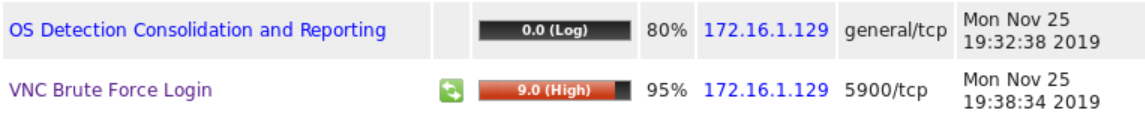
\includegraphics[scale = 0.4]{beforeVNC.png}}

  \caption {VNC Server com a password 'password'}

  \label {fig3}

\end{figure}
\begin{figure}[H]

  \centering

  \hbox{\hspace{-6em} \includegraphics[scale = 0.4]{afterVNC.png}}

  \caption {VNC Server com a password '5?V=X\#\&k'}

  \label {fig3}

\end{figure}
\item Vulnerabilidades extra corrigidas:
\end{itemize}
